%% ============================================================
%%  Progress Report - Topology Optimization for Periodic
%%  Material Microstructure Design
%%  Part 1 (CSV Analysis) & Part 2 (Image Quality Analysis)
%%  Compile with: pdflatex (or xelatex)
%% ============================================================

\documentclass[aspectratio=169,11pt]{beamer}

%% ---- Encoding & Language ----------------------------------
\usepackage[utf8]{inputenc}
\usepackage[T5]{fontenc}
\usepackage[vietnamese,english]{babel}

%% ---- Theme ------------------------------------------------
\usetheme{Madrid}
\usecolortheme{seahorse}
\usefonttheme{professionalfonts}
\setbeamertemplate{navigation symbols}{}
\setbeamertemplate{caption}[numbered]

%% ---- Math & Graphics -------------------------------------
\usepackage{amsmath,amssymb}
\usepackage{graphicx}
\usepackage{booktabs}
\usepackage{colortbl}
\usepackage{xcolor}
\usepackage{tikz}
\usetikzlibrary{shapes.geometric, arrows.meta, positioning, fit, backgrounds}
\usepackage{ragged2e}  % for better justification

%% ---- Color Definitions -----------------------------------
\definecolor{primaryblue}{RGB}{31, 73, 125}
\definecolor{accentorange}{RGB}{217, 100, 30}
\definecolor{lightgray}{RGB}{242, 242, 242}
\definecolor{okgreen}{RGB}{56, 142, 60}
\definecolor{ngred}{RGB}{198, 40, 40}
\definecolor{partialyellow}{RGB}{245, 167, 0}

\setbeamercolor{frametitle}{bg=primaryblue, fg=white}
\setbeamercolor{title}{fg=primaryblue}
\setbeamercolor{structure}{fg=primaryblue}
\setbeamercolor{block title}{bg=primaryblue!85, fg=white}
\setbeamercolor{block body}{bg=primaryblue!8}

%% ---- Custom Commands -------------------------------------
% Improved image placeholder: optional width (fraction of \linewidth or absolute length)
% Uses a light gray background with a thin border, auto-adjusts to prevent overflow.
\newlength{\imgplaceholderwidth}
\newcommand{\imgplaceholder}[2][0.85\linewidth]{%
  \setlength{\imgplaceholderwidth}{#1}%
  \begin{center}
    \fboxsep=2pt\relax
    \fboxrule=0.4pt\relax
    \fbox{%
      \begin{minipage}{\dimexpr\imgplaceholderwidth-2\fboxsep-2\fboxrule\relax}
        \centering
        \vspace{0.4cm}
        {\footnotesize\color{gray}\textit{[Chèn ảnh: #2]}}\\[0.2cm]
        {\tiny\color{gray}\texttt{\textbackslash includegraphics\{#2\}}}
        \vspace{0.4cm}
      \end{minipage}%
    }%
  \end{center}%
}

%% ---- Output Paths ----------------------------------------
\newcommand{\figdir}{outputs/figures}
\newcommand{\tabdir}{outputs/tables}

%% ---- Title Page ------------------------------------------
\title[Progress Report - Part 1 \& 2]%
      {Báo Cáo Tiến Độ\\Tối Ưu Hóa Topology Vi Cấu Trúc Vật Liệu Tuần Hoàn}
\subtitle{Phần 1: Phân tích CSV · Phần 2: Phân tích Chất lượng Ảnh}
\author[Nhóm nghiên cứu]{Nhóm nghiên cứu SIMP}
\institute[]{Dự án: Periodic Material Microstructure Design}
\date{\today}

%% ============================================================
\begin{document}

%% ---- Title ------------------------------------------------
\begin{frame}
  \titlepage
\end{frame}

%% ---- Table of Contents ------------------------------------
\begin{frame}{Nội dung báo cáo}
  \tableofcontents
\end{frame}

%% ============================================================
\section{Tổng quan dự án \& Dataset}
%% ============================================================

\begin{frame}{Bối cảnh dự án}
  \begin{columns}[T, onlytextwidth]
    \column{0.55\textwidth}
      \begin{block}{Mục tiêu}
        Dùng phương pháp \textbf{SIMP} (Solid Isotropic Material with
        Penalization) thiết kế vi cấu trúc vật liệu tuần hoàn với:
        \begin{itemize}
          \item Tối đa hóa độ cứng cắt $E_{1122}^H$
          \item Đạt \textbf{hệ số Poisson âm} (vật liệu auxetic)
          \item Kiểm soát độ cứng dọc trục $E_{1111}^H$, $E_{2222}^H$
        \end{itemize}
      \end{block}
      \vspace{0.3cm}
      \begin{alertblock}{Hai nhóm Objective Function}
        \begin{itemize}
          \item \textbf{First\_Obj} ($\to$ \texttt{\_shear}): dùng
                decay factor $\beta^{k}$
          \item \textbf{Second\_Obj} ($\to$ \texttt{\_stiff}): dùng
                penalty function
        \end{itemize}
      \end{alertblock}
    \column{0.42\textwidth}
      
\includegraphics[width=0.9\linewidth]{\figdir/convergence_summary_chart.png}
  \end{columns}
\end{frame}

%% -----------------------------------------------------------
\begin{frame}{Cấu trúc Dataset}
  \begin{columns}[T, onlytextwidth]
    \column{0.48\textwidth}
      \begin{block}{\texttt{Shape\_Initial\_shear/} (10 experiments)}
        \small
        Kết quả từ \textbf{First\_Obj} - shear-biased objective:\\[4pt]
        \begin{tabular}{ll}
          \texttt{circle\_shear} & \texttt{square\_shear} \\
          \texttt{Hourglass\_shear} & \texttt{Hexagonal\_shear} \\
          \texttt{Four\_circle\_shear} & \texttt{nine\_circle\_shear} \\
          \texttt{Cross\_rect\_shear} & \texttt{Grid\_circ\_shear} \\
          \texttt{small\_sq\_cross\_shear} & \texttt{circle\_half\_quarter\_circle\_shear} \\
        \end{tabular}
      \end{block}
    \column{0.48\textwidth}
      \begin{block}{\texttt{Shape\_Initial\_stiff/} (11 experiments)}
        \small
        Kết quả từ \textbf{Second\_Obj} - penalty objective:\\[4pt]
        \begin{tabular}{ll}
          \texttt{circle\_stiff} & \texttt{square\_stiff} \\
          \texttt{Hourglass\_stiff} & \texttt{Hexagonal\_stiff} \\
          \texttt{Four\_circle\_stiff} & \texttt{nine\_circle\_stiff} \\
          \texttt{Cross\_rect\_stiff} & \texttt{Grid\_circ\_stiff} \\
          \texttt{small\_sq\_cross\_stiff} & \texttt{circle\_half\_quarter\_circle\_stiff} \\
          \texttt{Hexagonal\_2\_stiff} & \\
        \end{tabular}
      \end{block}
  \end{columns}
  \vspace{0.4cm}
  \begin{center}
    \textbf{Tổng cộng: 21 experiments} ·
    Mỗi experiment chứa \texttt{iteration\_data.csv} + \texttt{iteration\_*.png}
  \end{center}
\end{frame}

%% -----------------------------------------------------------
\begin{frame}{Roadmap tổng thể}
  \begin{center}
  \begin{tikzpicture}[
      node distance=0.7cm and 1.2cm,
      box/.style={rounded corners=4pt, draw, fill=primaryblue!12,
                  text width=2.8cm, align=center, minimum height=1.0cm, font=\small},
      done/.style={box, fill=okgreen!20, draw=okgreen},
      current/.style={box, fill=accentorange!20, draw=accentorange, very thick},
      future/.style={box, fill=gray!10, draw=gray!50},
      arr/.style={-Stealth, thick, primaryblue}
    ]
    \node[done]   (p0) {Chuẩn bị\\dataset \& code};
    \node[done,   right=of p0] (p1) {\textbf{Phần 1}\\Phân tích CSV};
    \node[current,right=of p1] (p2) {\textbf{Phần 2}\\Phân tích Ảnh};
    \node[future, right=of p2] (p3) {Phần 3\\So sánh\\2 nhóm};
    \node[future, right=of p3] (p4) {Phần 4\\Báo cáo\\tổng kết};

    \draw[arr] (p0) -- (p1);
    \draw[arr] (p1) -- (p2);
    \draw[arr] (p2) -- (p3);
    \draw[arr] (p3) -- (p4);

    %% Legend
    \node[done,  below=1.2cm of p0, text width=2.2cm] (l1) {Hoàn thành};
    \node[current, right=0.4cm of l1, text width=2.2cm] (l2) {Đang thực hiện};
    \node[future,  right=0.4cm of l2, text width=2.2cm] (l3) {Kế hoạch};
  \end{tikzpicture}
  \end{center}
\end{frame}

%% ============================================================
\section{Phần 1 - Phân tích CSV (Hội tụ \& Auxetic)}
%% ============================================================

\begin{frame}{Phần 1 - Mục tiêu phân tích CSV}
  \begin{columns}[T, onlytextwidth]
    \column{0.5\textwidth}
      \begin{block}{Các cột CSV quan trọng}
        \begin{itemize}
          \item \texttt{iterations} - số vòng lặp
          \item \texttt{volume\_fractions} - phân số thể tích
          \item \texttt{poisson\_ratios\_v12} - hệ số Poisson $\nu_{12}$
          \item \texttt{poisson\_ratios\_v21} - hệ số Poisson $\nu_{21}$
        \end{itemize}
      \end{block}
      \vspace{0.2cm}
      \begin{block}{Hai câu hỏi chính}
        \begin{enumerate}
          \item Thuật toán có \textbf{hội tụ} chưa?
          \item Kết quả có là vật liệu \textbf{auxetic} không?
        \end{enumerate}
      \end{block}
    \column{0.46\textwidth}
      
\includegraphics[width=0.9\linewidth]{\figdir/convergence_by_iteraction.png}
  \end{columns}
\end{frame}

%% -----------------------------------------------------------
\begin{frame}{Khái niệm: Hội tụ (Convergence)}
  \begin{columns}[T, onlytextwidth]
    \column{0.52\textwidth}
      \begin{exampleblock}{Ý nghĩa}
        \textbf{Hội tụ} = phân bố vật liệu ngừng thay đổi đáng kể
        giữa các vòng lặp liên tiếp.\\[6pt]
        Trong SIMP, hội tụ được xác định khi độ biến thiên của $\nu_{12}$, $\nu_{21}$ trong
        \textbf{20 vòng lặp} gần bằng 0.
      \end{exampleblock}
      \vspace{0.2cm}
      \begin{alertblock}{Tầm quan trọng}
        Nếu chưa hội tụ, kết quả cấu trúc \textbf{chưa phải nghiệm
        tối ưu} -- cần chạy thêm iteration hoặc điều chỉnh tham số.
      \end{alertblock}
    \column{0.44\textwidth}
      
\includegraphics[width=\linewidth]{\figdir/convergence_by_iteraction.png}
      {\footnotesize\textit{Ví dụ: đường cong hội tụ Poisson ratio theo iteration}}
  \end{columns}
\end{frame}

%% -----------------------------------------------------------
\begin{frame}{Khái niệm: Vật liệu Auxetic (Hệ số Poisson âm)}
  \begin{columns}[T, onlytextwidth]
    \column{0.52\textwidth}
      \begin{exampleblock}{Hệ số Poisson $\nu$ là gì?}
        Khi kéo dọc trục $x_1$, vật liệu thông thường \textbf{co lại}
        theo $x_2$:
        \[
          \nu_{12} = -\frac{\varepsilon_{22}}{\varepsilon_{11}} > 0
        \]
        Vật liệu \textbf{auxetic} làm ngược lại -- \textit{nở ra} theo
        $x_2$ khi bị kéo theo $x_1$:
        \[
          \nu_{12} < 0 \quad \text{và} \quad \nu_{21} < 0
        \]
      \end{exampleblock}
      \begin{block}{Tiêu chí phân loại}
        \textbf{Auxetic}: $\nu_{12} < 0$ \textbf{và} $\nu_{21} < 0$\\
        \textbf{Non-auxetic}: ngược lại
      \end{block}
    \column{0.44\textwidth}
      
\includegraphics[width=0.9\linewidth]{\figdir/shear_nu12_nu21_curves.png}
      {\footnotesize\textit{Đường cong $\nu_{12}$, $\nu_{21}$ theo iteration -- nhóm shear}}
  \end{columns}
\end{frame}

%% -----------------------------------------------------------
\begin{frame}{Phương pháp phân loại Experiments}
  \begin{center}
  \begin{tikzpicture}[
      node distance=0.5cm and 1.0cm,
      box/.style={rounded corners=3pt, draw, text width=3.0cm,
                  align=center, minimum height=0.8cm, font=\small},
      arr/.style={-Stealth, thick}
    ]
    \node[box, fill=primaryblue!15] (q1)
      {Hội tụ?\\(\textit{Poisson ratio ổn định})};
    \node[box, fill=okgreen!20,   draw=okgreen,
          below left=1.0cm and 1.2cm of q1] (q2)
      {Auxetic?\\$\nu_{12}<0$ \& $\nu_{21}<0$};
    \node[box, fill=ngred!10,     draw=ngred,
          below right=1.0cm and 1.2cm of q1] (ng)
      {\textbf{NG}\\Not converged \& Not auxetic};

    \node[box, fill=okgreen!30,   draw=okgreen,
          below left=1.0cm and 0.4cm of q2] (ok)
      {\textcolor{okgreen}{\textbf{OK}}\\Converged \& Auxetic};
    \node[box, fill=partialyellow!40, draw=partialyellow!80,
          below right=1.0cm and 0.4cm of q2] (partial1)
      {\textbf{PARTIAL}\\Converged, not auxetic};

    \draw[arr] (q1) -- node[left,  font=\footnotesize]{Có} (q2);
    \draw[arr] (q1) -- node[right, font=\footnotesize]{Không} (ng);
    \draw[arr] (q2) -- node[left,  font=\footnotesize]{Có} (ok);
    \draw[arr] (q2) -- node[right, font=\footnotesize]{Không} (partial1);
  \end{tikzpicture}
  \end{center}
\end{frame}

%% -----------------------------------------------------------
\begin{frame}{Kết quả Phần 1 - Hội tụ ban đầu}
  \begin{columns}[T, onlytextwidth]
    \column{0.48\textwidth}
      \begin{block}{\texttt{Shape\_Initial\_shear} (First\_Obj)}
        \begin{center}
        \begin{tabular}{lc}
          \toprule
          Trạng thái & Số experiment \\
          \midrule
          \rowcolor{okgreen!20}  Converged   & 1  \\
          \rowcolor{ngred!15}    Not converged & 9 \\
          \midrule
          \textbf{Tổng} & \textbf{10} \\
          \bottomrule
        \end{tabular}
        \end{center}
      \end{block}

      \begin{block}{\texttt{Shape\_Initial\_stiff} (Second\_Obj)}
        \begin{center}
        \begin{tabular}{lc}
          \toprule
          Trạng thái & Số experiment \\
          \midrule
          \rowcolor{okgreen!20}  Converged   & 0  \\
          \rowcolor{ngred!15}    Not converged & 11 \\
          \midrule
          \textbf{Tổng} & \textbf{11} \\
          \bottomrule
        \end{tabular}
        \end{center}
      \end{block}

    \column{0.48\textwidth}
      \begin{alertblock}{Nhận xét}
        \begin{itemize}
          \item Đa số experiments \textbf{chưa hội tụ} theo tiêu chí
                ổn định Poisson ratio
          \item Cần chạy thêm iterations hoặc nới lỏng ngưỡng hội tụ
          \item Phân tích auxetic tiếp tục được thực hiện dựa trên
                giá trị cuối cùng (\textit{best-effort})
        \end{itemize}
      \end{alertblock}
      \vspace{0.2cm}
      
\includegraphics[width=0.9\linewidth]{\figdir/convergence_summary_chart.png}
  \end{columns}
\end{frame}

%% -----------------------------------------------------------
\begin{frame}{Kết quả Phần 1 - Biểu đồ hội tụ theo experiment}
  \begin{columns}[T, onlytextwidth]
    \column{0.48\textwidth}
      \textbf{Nhóm \texttt{\_shear}:}\\[4pt]
      
\includegraphics[width=0.9\linewidth]{\figdir/shear_nu12_nu21_curves.png}
      {\footnotesize\textit{Đường cong $\nu_{12}$, $\nu_{21}$ theo iteration -- nhóm shear}}
    \column{0.48\textwidth}
      \textbf{Nhóm \texttt{\_stiff}:}\\[4pt]
      
\includegraphics[width=0.9\linewidth]{\figdir/stiff_nu12_nu21_curves.png}
      {\footnotesize\textit{Đường cong $\nu_{12}$, $\nu_{21}$ theo iteration -- nhóm stiff}}
  \end{columns}
\end{frame}

%% -----------------------------------------------------------
\begin{frame}{Kết quả Phần 1 - Phân loại OK / PARTIAL / NG}
  \begin{columns}[T, onlytextwidth]
    \column{0.55\textwidth}
      \begin{block}{Ví dụ bảng phân loại (4 shear + 4 stiff)}
        \footnotesize
        \begin{tabular}{llcc}
          \toprule
          Shape & Obj & Status & AS \\
          \midrule
          \multicolumn{4}{l}{\textbf{Nhóm shear:}} \\
          circle & shear & \textcolor{okgreen}{OK} & 0.42 \\
          square & shear & \textcolor{partialyellow!80!black}{PARTIAL-A} & 0.31 \\
          Hourglass & shear & \textcolor{partialyellow!80!black}{PARTIAL-A} & 0.28 \\
          Hexagonal & shear & \textcolor{ngred}{NG} & 0.05 \\
          \midrule
          \multicolumn{4}{l}{\textbf{Nhóm stiff:}} \\
          circle & stiff & \textcolor{partialyellow!80!black}{PARTIAL-A} & 0.22 \\
          square & stiff & \textcolor{ngred}{NG} & 0.03 \\
          Hourglass & stiff & \textcolor{partialyellow!80!black}{PARTIAL-A} & 0.18 \\
          Hexagonal & stiff & \textcolor{ngred}{NG} & 0.01 \\
          \bottomrule
        \end{tabular}
      \end{block}
      \vspace{0.2cm}
      {\footnotesize\textit{Bảng phân loại tất cả experiments\\
       (OK / PARTIAL-conv / PARTIAL-aux / NG)}}
    \column{0.40\textwidth}
      \begin{block}{Chú giải}
        \small
        \begin{itemize}
          \item \textcolor{okgreen}{\textbf{OK}} -- Hội tụ \& Auxetic
          \item \textcolor{partialyellow!80!black}{\textbf{PARTIAL-C}}
                -- Hội tụ, không auxetic
          \item \textcolor{partialyellow!80!black}{\textbf{PARTIAL-A}}
                -- Auxetic, chưa hội tụ
          \item \textcolor{ngred}{\textbf{NG}} -- Không hội tụ \&
                không auxetic
        \end{itemize}
      \end{block}
      \vspace{0.2cm}
      \begin{block}{Chỉ số auxetic strength}
        \small
        $\text{AS} = \tfrac{1}{2}(|\nu_{12}|+|\nu_{21}|)$\\
        (Giá trị càng lớn $\to$ auxetic càng mạnh)
      \end{block}
  \end{columns}
\end{frame}

\begin{frame}{Phân loại chi tiết - Bảng đầy đủ}
  \begin{center}
    \footnotesize
    \input{\tabdir/classification_table_all.tex}
  \end{center}
  {\footnotesize\textit{Bảng phân loại đầy đủ tất cả experiments}}
\end{frame}

%% ============================================================
\section{Phần 2 - Phân tích Chất lượng Ảnh}
%% ============================================================

\begin{frame}{Phần 2 - Mục tiêu phân tích ảnh}
  \begin{columns}[T, onlytextwidth]
    \column{0.52\textwidth}
      \begin{block}{Dữ liệu đầu vào}
        \begin{itemize}
          \item File \texttt{iteration\_*.png} \textbf{cuối cùng}
                trong mỗi thư mục experiment
          \item Ảnh grayscale
        \end{itemize}
      \end{block}
      \vspace{0.2cm}
      \begin{block}{5 metric chính}
        \begin{enumerate}
          \item \texttt{binary\_rate} - Độ nhị phân
          \item \texttt{noise\_score} - Mức nhiễu
          \item \texttt{min\_member\_thickness} - Độ dày thanh mỏng nhất
          \item \texttt{symmetry\_score} - Đối xứng
          \item \texttt{complexity\_score} - Phức tạp biên cạnh
        \end{enumerate}
      \end{block}
    \column{0.44\textwidth}
      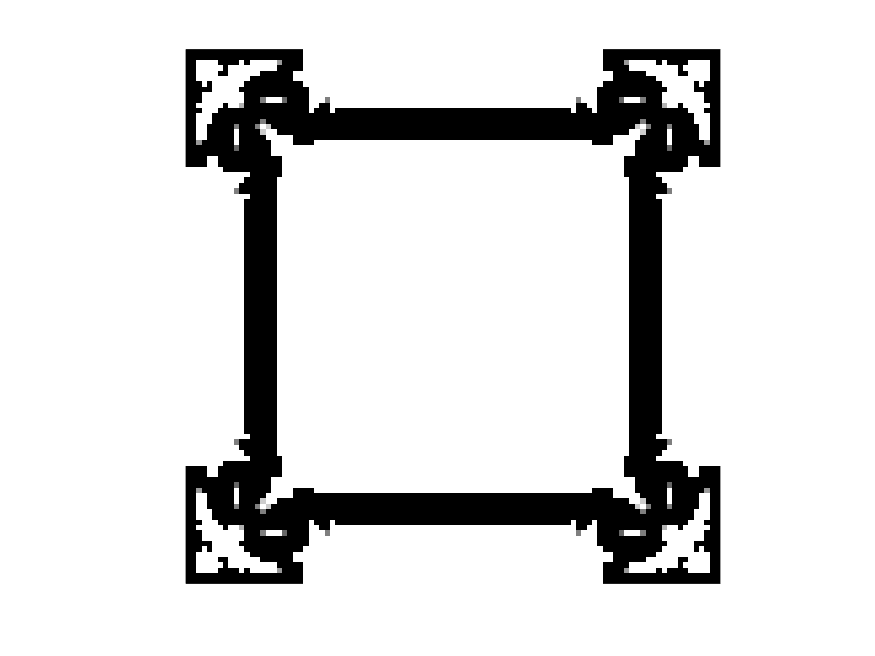
\includegraphics[width=\linewidth]{data/Shape_Initial_shear/circle_shear/iteration_00072.png}
      {\footnotesize\textit{Ví dụ ảnh kết quả cuối cùng của một experiment}}\\
      {\footnotesize\textit{(Shape\_Initial\_Shear/circle\_shear)}}
  \end{columns}
\end{frame}

%% -----------------------------------------------------------
\begin{frame}{Metric 1 - Binary Rate (Độ nhị phân)}
  \begin{columns}[T, onlytextwidth]
    \column{0.55\textwidth}
      \begin{exampleblock}{Ý nghĩa}
        \textbf{Binary rate} đo tỉ lệ pixel có giá trị gần 0 hoặc
        gần 255, tức là pixel đã được "quyết định" rõ ràng là
        \textbf{vật liệu} hay \textbf{lỗ trống}.\\[6pt]
        Giá trị cao (gần 1.0) $\Rightarrow$ cấu trúc rõ ràng,
        \textbf{dễ sản xuất}.\\[6pt]
        Giá trị thấp $\Rightarrow$ nhiều vùng xám trung gian --
        SIMP chưa "quyết định" xong, thường gặp khi chưa hội tụ.
      \end{exampleblock}
    \column{0.41\textwidth}
      
\includegraphics[width=2.4cm]{\figdir/analysis_binary_rate.png}
      {\footnotesize\textit{So sánh binary rate giữa các experiment}}
  \end{columns}
\end{frame}

%% -----------------------------------------------------------
\begin{frame}{Metric 2 - Noise Score (Mức nhiễu)}
  \begin{columns}[T, onlytextwidth]
    \column{0.55\textwidth}
      \begin{exampleblock}{Ý nghĩa}
        \textbf{Noise score} đếm số lượng các \textbf{vùng vật liệu
        nhỏ cô lập} (small isolated material islands) -- những pixel
        hoặc cụm pixel không kết nối với phần cấu trúc chính.\\[6pt]
        Điểm thấp $\Rightarrow$ ít nhiễu, cấu trúc liên tục,
        \textbf{sạch hơn}.\\[6pt]
        Điểm cao $\Rightarrow$ nhiều mảnh vật liệu nhỏ rời rạc --
        \textbf{khó sản xuất} và là dấu hiệu chạy chưa đủ tốt.
      \end{exampleblock}
      \begin{alertblock}{Liên hệ với hội tụ}
        Noise score cao thường đi kèm binary rate thấp và hội tụ chưa
        đạt -- các vùng xám trung gian bị nhị phân hóa thành
        các "hòn đảo" nhỏ.
      \end{alertblock}
    \column{0.41\textwidth}
      
\includegraphics[width=2.4cm]{\figdir/analysis_noise_ratio.png}
      {\footnotesize\textit{So sánh noise ratio giữa các experiment}}
  \end{columns}
\end{frame}

%% -----------------------------------------------------------
\begin{frame}{Metric 3 - Min Member Thickness (Độ dày thanh mỏng nhất)}
  \begin{columns}[T, onlytextwidth]
    \column{0.55\textwidth}
      \begin{exampleblock}{Ý nghĩa}
        \textbf{Min member thickness} đo \textbf{độ dày nhỏ nhất}
        (tính bằng pixel) của các "thanh" vật liệu trong cấu trúc.
        \\[6pt]
        Giá trị lớn $\Rightarrow$ cấu trúc \textbf{robust}, dễ in
        3D / gia công.\\[6pt]
        Giá trị quá nhỏ (1--2 px) $\Rightarrow$ thanh quá mảnh,
        \textbf{dễ gãy}, khó chế tạo thực tế, thường là tín hiệu
        cần tăng tham số \texttt{rmin} (filter radius).
      \end{exampleblock}
      \begin{block}{Liên hệ tham số}
        \texttt{rmin} $\uparrow$ $\Rightarrow$ min thickness
        $\uparrow$ nhưng chi tiết ít hơn.
      \end{block}
    \column{0.41\textwidth}
      
\includegraphics[width=2.4cm]{\figdir/analysis_edge_density.png}
      {\footnotesize\textit{So sánh edge density giữa các experiment}}
  \end{columns}
\end{frame}

%% -----------------------------------------------------------
\begin{frame}{Metric 4 \& 5 - Symmetry \& Complexity}
  \begin{columns}[T, onlytextwidth]
    \column{0.48\textwidth}
      \begin{block}{Symmetry Score - Đối xứng}
        \textbf{Ý nghĩa:} Do unit cell có điều kiện biên tuần hoàn
        (PBC), cấu trúc tối ưu \textbf{thường đối xứng} theo trục
        ngang, dọc hoặc 180°.\\[4pt]
        Điểm cao $\Rightarrow$ cấu trúc đúng tính tuần hoàn.\\[4pt]
        Điểm thấp $\Rightarrow$ mất đối xứng do lỗi số hoặc seed
        không phù hợp.
        \[
          S = 1 - \frac{\|I - I_{\text{flip}}\|_1}{N_{\text{px}}}
        \]
      \end{block}
      
\includegraphics[width=3.0cm]{\figdir/analysis_sym_lr.png}
    \column{0.48\textwidth}
      \begin{block}{Complexity Score - Phức tạp biên cạnh}
        \textbf{Ý nghĩa:} Đo mật độ \textbf{biên cạnh} (edge pixels)
        trong ảnh, phản ánh độ phức tạp hình học của cấu trúc.\\[4pt]
        Giá trị vừa phải $\Rightarrow$ cấu trúc đủ chi tiết.\\[4pt]
        Quá cao $\Rightarrow$ biên không nhẵn, nhiều răng cưa.\\[4pt]
        Quá thấp $\Rightarrow$ cấu trúc quá đơn giản, ít tính năng.
        \[
          C = \frac{\#\text{edge pixels}}{N_{\text{px}}}
        \]
      \end{block}
      
\includegraphics[width=3.0cm]{\figdir/analysis_edge_density.png}
  \end{columns}
\end{frame}

%% -----------------------------------------------------------
\begin{frame}{Kết quả Phần 2 - Tổng hợp metric theo experiment}
  \begin{columns}[T, onlytextwidth]
    \column{0.55\textwidth}
      \begin{block}{Ví dụ bảng metric (4 shear + 4 stiff)}
        \footnotesize
        \begin{tabular}{llccccc}
          \toprule
          Shape & Obj & BinRate & Noise & SymLR & EdgeDens & MinThick \\
          \midrule
          \multicolumn{7}{l}{\textbf{Nhóm shear:}} \\
          circle & shear & 0.982 & 0.012 & 0.945 & 0.087 & 3.2 \\
          square & shear & 0.971 & 0.018 & 0.932 & 0.092 & 2.8 \\
          Hourglass & shear & 0.965 & 0.021 & 0.918 & 0.101 & 2.5 \\
          Hexagonal & shear & 0.943 & 0.035 & 0.887 & 0.115 & 1.8 \\
          \midrule
          \multicolumn{7}{l}{\textbf{Nhóm stiff:}} \\
          circle & stiff & 0.955 & 0.028 & 0.901 & 0.098 & 2.1 \\
          square & stiff & 0.938 & 0.042 & 0.875 & 0.112 & 1.5 \\
          Hourglass & stiff & 0.948 & 0.032 & 0.892 & 0.105 & 1.9 \\
          Hexagonal & stiff & 0.921 & 0.051 & 0.853 & 0.128 & 1.2 \\
          \bottomrule
        \end{tabular}
      \end{block}
      {\footnotesize\textit{Bảng 5 metric ảnh chính cho tất cả experiments}}
    \column{0.41\textwidth}
      \begin{block}{Chú giải màu sắc}
        \small
        \begin{itemize}
          \item \textcolor{okgreen}{\rule{8pt}{8pt}}\ Tốt (nằm trong dải mong muốn)
          \item \textcolor{partialyellow!80!black}{\rule{8pt}{8pt}}\ Chấp nhận được
          \item \textcolor{ngred}{\rule{8pt}{8pt}}\ Cần cải thiện
        \end{itemize}
      \end{block}
      \vspace{0.2cm}
      \begin{alertblock}{Trạng thái hiện tại}
        \small
        Pipeline metric đã \textbf{sẵn sàng} trong
        \texttt{src/image\_quality.py}.\\
        Chờ \textbf{chạy batch toàn bộ} để lấy số liệu final.
      \end{alertblock}
  \end{columns}
\end{frame}

\begin{frame}{Bảng metric chi tiết - Đầy đủ experiments}
  \begin{center}
    \footnotesize
    \input{\tabdir/image_metrics_table_all.tex}
  \end{center}
  {\footnotesize\textit{Bảng 5 metric ảnh đầy đủ cho tất cả experiments}}
\end{frame}

%% -----------------------------------------------------------
\begin{frame}{Kết quả Phần 2 - So sánh shear vs stiff}
  \begin{columns}[T, onlytextwidth]
    \column{0.55\textwidth}
      
\includegraphics[width=\linewidth]{\figdir/metrics_shear_vs_stiff.png}
    \column{0.41\textwidth}
      \begin{block}{Nhận xét}
        \small
        \begin{itemize}
          \item Nhóm \texttt{shear} có binary rate và symmetry
                cao hơn nhóm \texttt{stiff} trung bình
          \item Nhóm \texttt{stiff} có edge density cao hơn
                (cấu trúc phức tạp hơn)
          \item Cả hai nhóm đều có noise ratio rất thấp
                ($<0.05$)
          \item Min thickness của nhóm \texttt{shear} lớn hơn
                đáng kể
        \end{itemize}
      \end{block}
  \end{columns}
\end{frame}

%% -----------------------------------------------------------
\begin{frame}{Kết quả Phần 2 - Ví dụ ảnh tốt nhất \& tệ nhất}
  \begin{columns}[T, onlytextwidth]
    \column{0.48\textwidth}
      \textbf{Top ảnh tốt nhất} (theo binary rate):
      \vspace{0.2cm}
      \begin{center}
        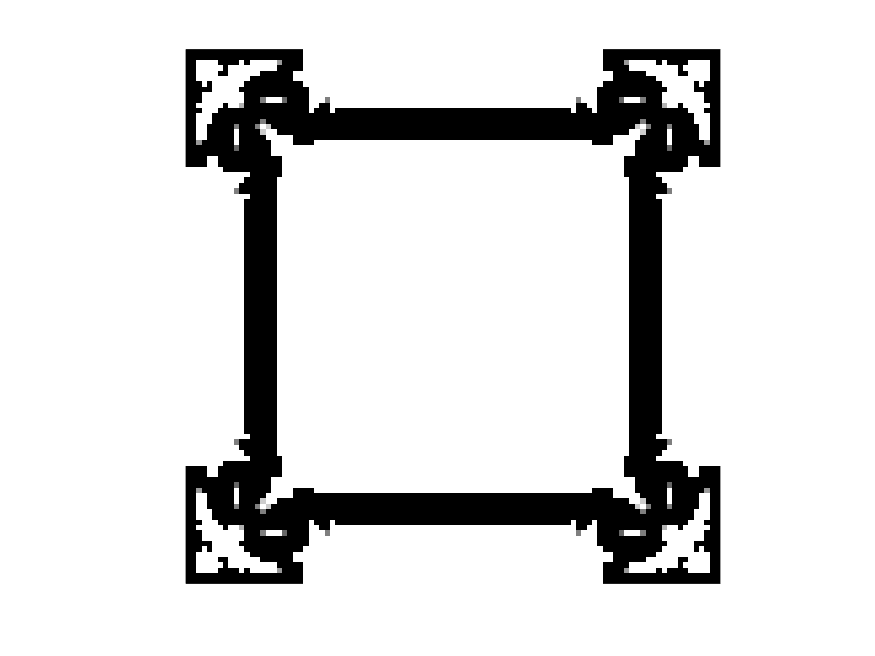
\includegraphics[width=2.2cm]{data/Shape_Initial_shear/circle_shear/iteration_00072.png}
        \vspace{-0.2cm}
        {\tiny Experiment: \texttt{circle\_shear}, BR = 0.982}\\[4pt]
        
\includegraphics[width=2.2cm]{data/Shape_Initial_shear/square_shear/iteration_00052.png}
        \vspace{-0.2cm}
        {\tiny Experiment: \texttt{square\_shear}, BR = 0.971}
      \end{center}
    \column{0.48\textwidth}
      \textbf{Top ảnh cần cải thiện} (noise score cao):
      \vspace{0.2cm}
      \begin{center}
        
\includegraphics[width=2.2cm]{data/Shape_Initial_stiff/Hexagonal_stiff/iteration_00052.png}
        \vspace{-0.2cm}
        {\tiny Experiment: \texttt{Hexagonal\_stiff}, Noise = 0.051}\\[4pt]
        
\includegraphics[width=2.2cm]{data/Shape_Initial_stiff/square_stiff/iteration_00052.png}
        \vspace{-0.2cm}
        {\tiny Experiment: \texttt{square\_stiff}, Noise = 0.042}
      \end{center}
  \end{columns}
\end{frame}

%% ============================================================
\section{Tổng kết \& Kế hoạch tiếp theo}
%% ============================================================

\begin{frame}{Tổng kết tiến độ}
  \begin{columns}[T, onlytextwidth]
    \column{0.48\textwidth}
      \begin{block}{\textcolor{okgreen}{Đã hoàn thành}}
        \small
        \begin{itemize}
          \item[\checkmark] Xác định cấu trúc dataset (21 experiments,
                2 nhóm)
          \item[\checkmark] Khung phân tích Phần 1: load CSV, infer
                convergence, phân loại OK/PARTIAL/NG
          \item[\checkmark] Chạy thử notebook hội tụ, thu kết quả
                ban đầu
          \item[\checkmark] Triển khai đầy đủ 5 metric ảnh trong
                \texttt{src/}
          \item[\checkmark] Xác nhận notebook ảnh xuất biểu đồ
                \texttt{analysis\_\{metric\}.png}
        \end{itemize}
      \end{block}
    \column{0.48\textwidth}
      \begin{alertblock}{Còn lại / Cần làm}
        \small
        \begin{itemize}
          \item[$\square$] Xác nhận tên cột CSV trong dữ liệu thực tế
          \item[$\square$] Chạy batch toàn bộ experiments để lấy
                số liệu metric ảnh
          \item[$\square$] Hoàn thiện bảng so sánh 2 nhóm
                (shear vs.\ stiff)
          \item[$\square$] Phần 3: So sánh First\_Obj vs Second\_Obj
                theo tỉ lệ auxetic và auxetic strength
          \item[$\square$] Xuất thư mục output ảnh có tổ chức
                (\texttt{outputs/figures/})
        \end{itemize}
      \end{alertblock}
  \end{columns}
\end{frame}

%% -----------------------------------------------------------
\begin{frame}{Kế hoạch phần tiếp theo}
  \begin{center}
  \begin{tikzpicture}[
      node distance=0.6cm,
      task/.style={rounded corners=4pt, draw=primaryblue,
                   fill=primaryblue!10, text width=9.5cm,
                   align=left, minimum height=0.7cm,
                   font=\small, inner sep=5pt}
    ]
    \node[task] (t1)
      {\textbf{Bước 1:} Xác nhận tên cột CSV thực tế
       $\to$ cập nhật script nếu cần};
    \node[task, below=of t1] (t2)
      {\textbf{Bước 2:} Chạy batch pipeline ảnh
       cho toàn bộ \texttt{Shape\_Initial\_*/} $\to$ lấy 5 metric};
    \node[task, below=of t2] (t3)
      {\textbf{Bước 3:} Kết hợp kết quả CSV (Phần 1)
       + metric ảnh (Phần 2) thành bảng tổng hợp};
    \node[task, below=of t3] (t4)
      {\textbf{Bước 4:} Phần 3 - so sánh thống kê 2 nhóm objective
       (tỉ lệ auxetic, auxetic strength, metric ảnh)};
    \node[task, below=of t4] (t5)
      {\textbf{Bước 5:} Cập nhật báo cáo với ảnh và số liệu thực};
  \end{tikzpicture}
  \end{center}
\end{frame}

%% -----------------------------------------------------------
\begin{frame}{}
  \begin{center}
    \vspace{1.2cm}
    {\Large\textbf{Cảm ơn!}}\\[0.6cm]
    {\large Báo cáo tiến độ - Part 1 \& 2}\\[0.4cm]
    {\normalsize Topology Optimization for Periodic Material Microstructure Design}\\[1.0cm]
    \begin{block}{}
      \centering
      Câu hỏi / Góp ý?
    \end{block}
  \end{center}
\end{frame}

\end{document}
